\documentclass[book.tex]{subfiles}
\begin{document}
This chapter describes the target hardware of Wolfenstein 3D. I thought it would be important to details the hardware limitations and assets of the machine. For simplicity it is abstracted as a pipeline taking user commands as entry and outputting images and audio resulting in something fun.\\
 \bigskip
\begin{figure}[H]
\centering
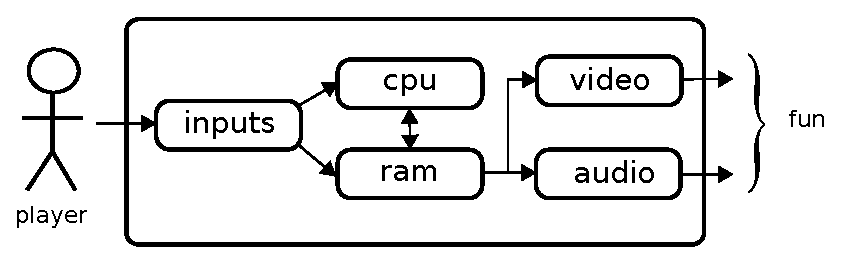
\includegraphics[scale=1.2]{imgs/fun_pipeline.eps}
%\def\svgscale{1.5}
%\input{imgs/fun_pipeline.pdf_tex}
\caption{Hardware pipeline.}
\label{fig:digraph}
\end{figure}

The pipeline comprises five stages. Some of them are bottlenecks for 3D game development while some are surprisingly good:

 \bigskip

\begin{figure}[H]
\centering
\begin{tabularx}{\textwidth}{ X X  }
  \toprule
  \textbf{Stage} & \textbf{Quality} \\ \bottomrule
  CPU & Poor \\ 
  RAM & Very Poor \\ 
  Video & Poor \\ 
  Audio & Good \\ 
  Inputs & Good \\ \bottomrule
\end{tabularx}
\caption{Pipeline stages.}  \label{fig:Pipeline stages}
\end{figure}

Overall, the pipeline offered a lot of resistance: hardware manufacturers had not embraced the game industry yet and it showed a lot. Ever since their inception in the 70s, IBM Personal Computers were designed to display static images and crunch integers. Real-time 3D, fractions and smooth sixty-frames-per-seconds animations were not on the blueprints.

\section{Central Processing Unit}
  \subsection{Overview}
  The ubiquitous CPU manufacturer was Intel with its x86 line of microprocessors.  The machines based on the 80286 released in 1982 were on the decline and progressively replaced by Intel's first 32 bits processor: The 80386. Moore's law was in full effect as can be seen on a mips\footnote{Million Instructions Per Second.} histogram:


\definecolor{skyblue1}{rgb}{0.1,0.624,0.812}


\begin{figure}[H]
\centering
  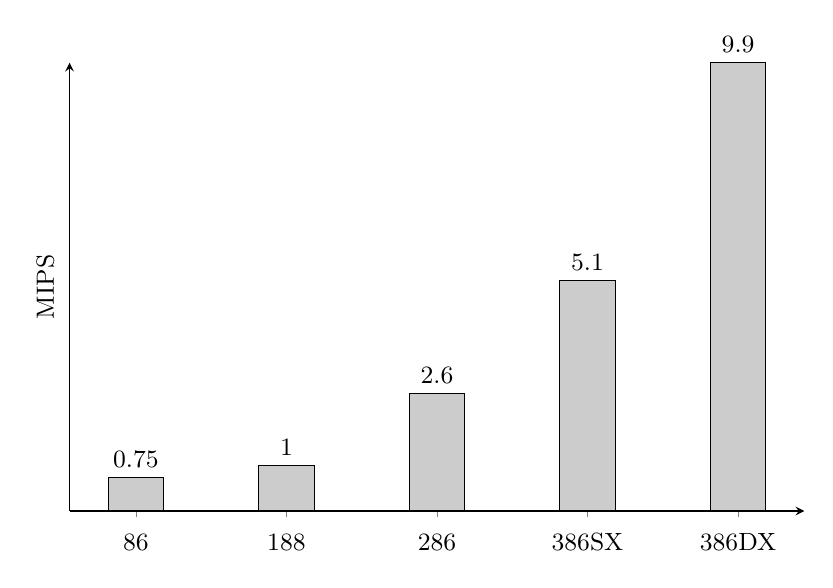
\begin{tikzpicture}[font=\small]
    \begin{axis}[
      width=0.9\textwidth,
      height=0.6\textwidth,
      ybar,
      bar width=20pt,
      ylabel={MIPS},
      ymin=0,
      ytick=\empty,
      xtick=data,
      axis x line=bottom,
      axis y line=left,
      enlarge x limits=0.11,
      symbolic x coords={86,188,286,386SX,386DX},
      xticklabel style={anchor=base,yshift=-\baselineskip},
      nodes near coords={\pgfmathprintnumber\pgfplotspointmeta}
    ]
      \addplot[fill=black!20,draw=black] coordinates {
        (86,0.75)
        (188,1)
        (286,2.6)
        (386SX,5.1)
        (386DX,9.9)
      };
    \end{axis}
    
   \end{tikzpicture}
   \caption{Processor speeds comparison.} \label{fig:mips}
 \end{figure}

 \textbf{\underline{Trivia :}} A modern processor such as the Intel Core i7 3.33 GHz operates at close to 180,000 Mips: Five orders of magnitude faster!

 \bigskip

\textbf{\underline{Trivia :}}  Two other companies were producing Intel clones: AMD and Cyrix. The mediocre performances did not justify the lower cost and as a result they never gathered a significant market share. Interestingly AMD evolved to become a serious challenger while Cyrix merged with National Semiconductor in 1997.

 \bigskip
 
 \textbf{\underline{Trivia :}} The 386SX and 386DX were identical processor. Yet the DX is twice faster than the SX thanks to a bus twice as wide (32 bits vs 16 bits) !












  \subsection{Floating Point}
  
  Wolfenstein 3D target machines were high-end 286 and low-end 386 machine. As seen previous those were powerful machines far outperforming any game console on the market. But all that power was not necessarily useful. In order to perform all the trigonometry it takes to perform three dimensional effects, the machines had to keep track of the fractional part of each operations. This is usually not an issue since the C language offers the types \codeword{float} and \codeword{double} precisely for that.\\
\\
It is important to understand what floating point is and how it works to fully grasp how useful it is when doing mathematics. \codeword{float} are 32 bits container following the IEEE 754 standard. Their purpose is store and allow operations on approximation of real numbers. The typical explanation is as follow: The 32 bits are divided in three sections:\\
\begin{itemize}
  \item One bit S for the sign.
  \item Seven bits E for the exponent.
  \item Twenty four bits for the mantissa.
\end{itemize} 

\begin{figure}[H]
\centering
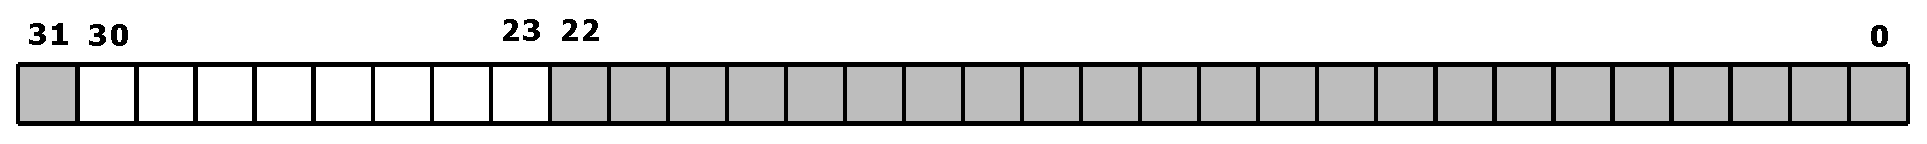
\includegraphics[scale=0.4]{imgs/floating_point_layout.eps}
\caption{Floating Point internals}
\label{fig:fp_internals}
\end{figure}
  \bigskip



\begin{figure}[H]
\centering
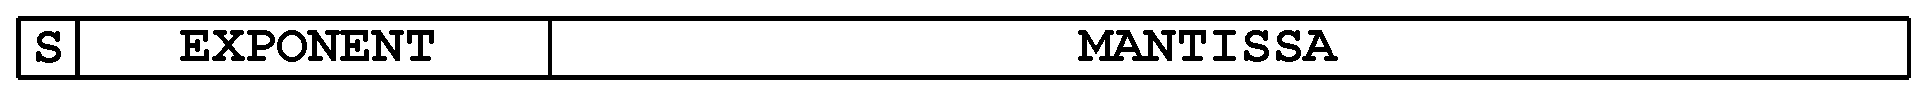
\includegraphics[scale=0.4]{imgs/floating_point_math.eps}
\caption{Floating Point three sections}
\label{fig:fp_regions}
\end{figure}
  \bigskip  


How numbers are stored and intepreted is usually explained with the formula \ref{eq:fp}).\


\begin{equation}\label{eq:fp}
\large
(-1)^S * 1.M * 2^{(E-127)}
\end{equation}
 
\bigskip  
Although correct, this way to explain floating point usually leaves programmers completely clueless. I blame this ignoble notation for discouraging generations of programmers, scaring them to the point they never looked back to understand how floating point actually works. Fortunately, there is a better way to explain it which involves a drawing and a slightly difference nomenclature. Instead of Exponent, think of a floating window between two consecutive power of two integers. And instead of a Mantissa think of an Offset within that window as in Figure \ref{fig:fp_internals}:
  
\begin{figure}[H]
\centering
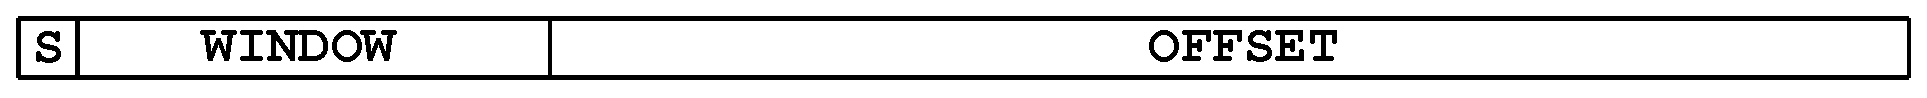
\includegraphics[scale=0.4]{imgs/floating_point_intuitive.eps}
\caption{Alternative Floating Point internals}
\label{fig:fp_internals}
\end{figure}
  \bigskip  

Figure \ref{fig:fp_internals_window} illustrate how the number 6.7 would be encoded, with the window starting at 4 (and therefore spanning up to next power of two: 8). The offset about 3/4 along the window.

\begin{figure}[H]
\centering
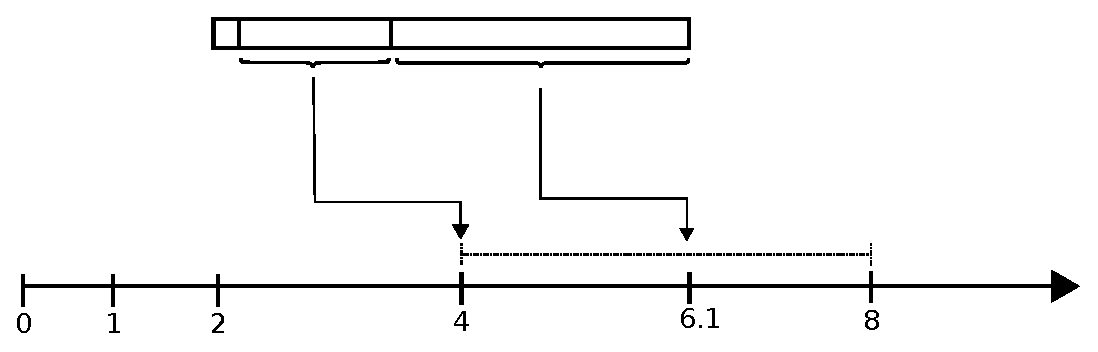
\includegraphics[scale=0.7]{imgs/floating_point_window.eps}

\caption{Value 6.7 approximated with floating point}
\label{fig:fp_internals_window}
\end{figure}
  \bigskip
  
Here is a detailled example which calculate the floating point representation of the number 3.14.
\begin{itemize}
 \item The number 3.14 is positive  $\rightarrow S=0$.
 \item The number 3.14 is between the power of two 2 and 4 so the floating window must start at $2^1$  $\rightarrow E=128$.
 \item Finally there are $2^{23}$ offsets available so 3.14 is at $\frac{4-3.14}{2} = 0.43 $. The mantissa/offset $\rightarrow M = 2^{23}*0.43 = 4781506$
\end{itemize}

Which in binary translate to:

\begin{itemize}
\item S = 0.
\item E = 10000000
\item M = 1001000111101111000011
\end{itemize}

\begin{figure}[H]
\centering
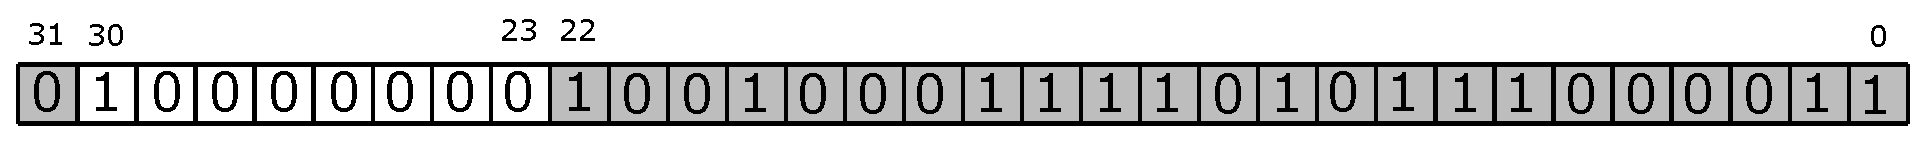
\includegraphics[scale=0.4]{imgs/floating_point_layout_pi.eps}
\caption{Floating Point internals}
\label{fig:fp_internals}
\end{figure}
  \bigskip

The value 3.14 is hemce approximated as 3.140000104904175.\\

The corresponding value with the ugly and useless formula:

\begin{equation}
3.14 = (-1)^0 * 1.57 * 2^{(128-127)}
\end{equation}

\bigskip

And finally the graphic representation:\\

\begin{figure}[H]
\centering
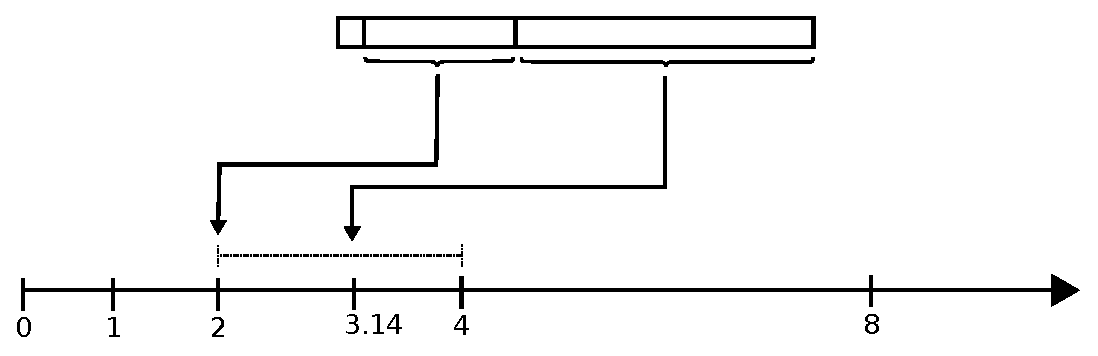
\includegraphics[scale=0.7]{imgs/floating_point_window_pi.eps}

\caption{3.14 window and offset.}
\label{fig:fp_internals}
\end{figure}
  \bigskip

If you (hopefully now) understand Floating Point, you can understand how handy it is to a 3D engine programmer.
Not only it approximate number very well, it also protect from overflow by floating the window when necessary.\\
\\
The representation is neat but computational intensive: To perform operation on two numbers is inherently expensive. In order to add, subtract, multiply or divide two numbers, they have to be expressed with the same window. Which mean converting one number to the representation used by the other usually with higher precision than 32 bits (typically 80 bits on Intel FPUs).\\
\\
This is not a problem when everything is hardwired...but it was a big problem for the 286 and the 386: \emph{They did not have a hardware Floating Point Unit}. Those operations were emulated in software by the compiler and therefore impossibly slow.\\
\bigskip
At first sight it looked like performing realtime trigonometry was out of the picture with 1992 machines unless a workaround could be found.

  \bigskip

 \textbf{\underline{Trivia :}} Since floating point units where so rare, why did the C language end up with a \codeword{float} and \codeword{double} types ? The machine used to invent it (PDP-11) did not have one either but the manufacturer (DEC) had promised Dennis Ritchie and Ken Thompson the next model would have one\footnote{The Development of the C Language by Dennis M. Ritchie}!

\bigskip  
\break
\textbf{\underline{Trivia :}} Some PCs did have hardware FPU. Intel sold what was marked as "Math CoProcessor". Intented to scientists, performances were average, price outrageous and sales mediocre :\\
\begin{figure}[H]
\centering
  \shadowbox{
      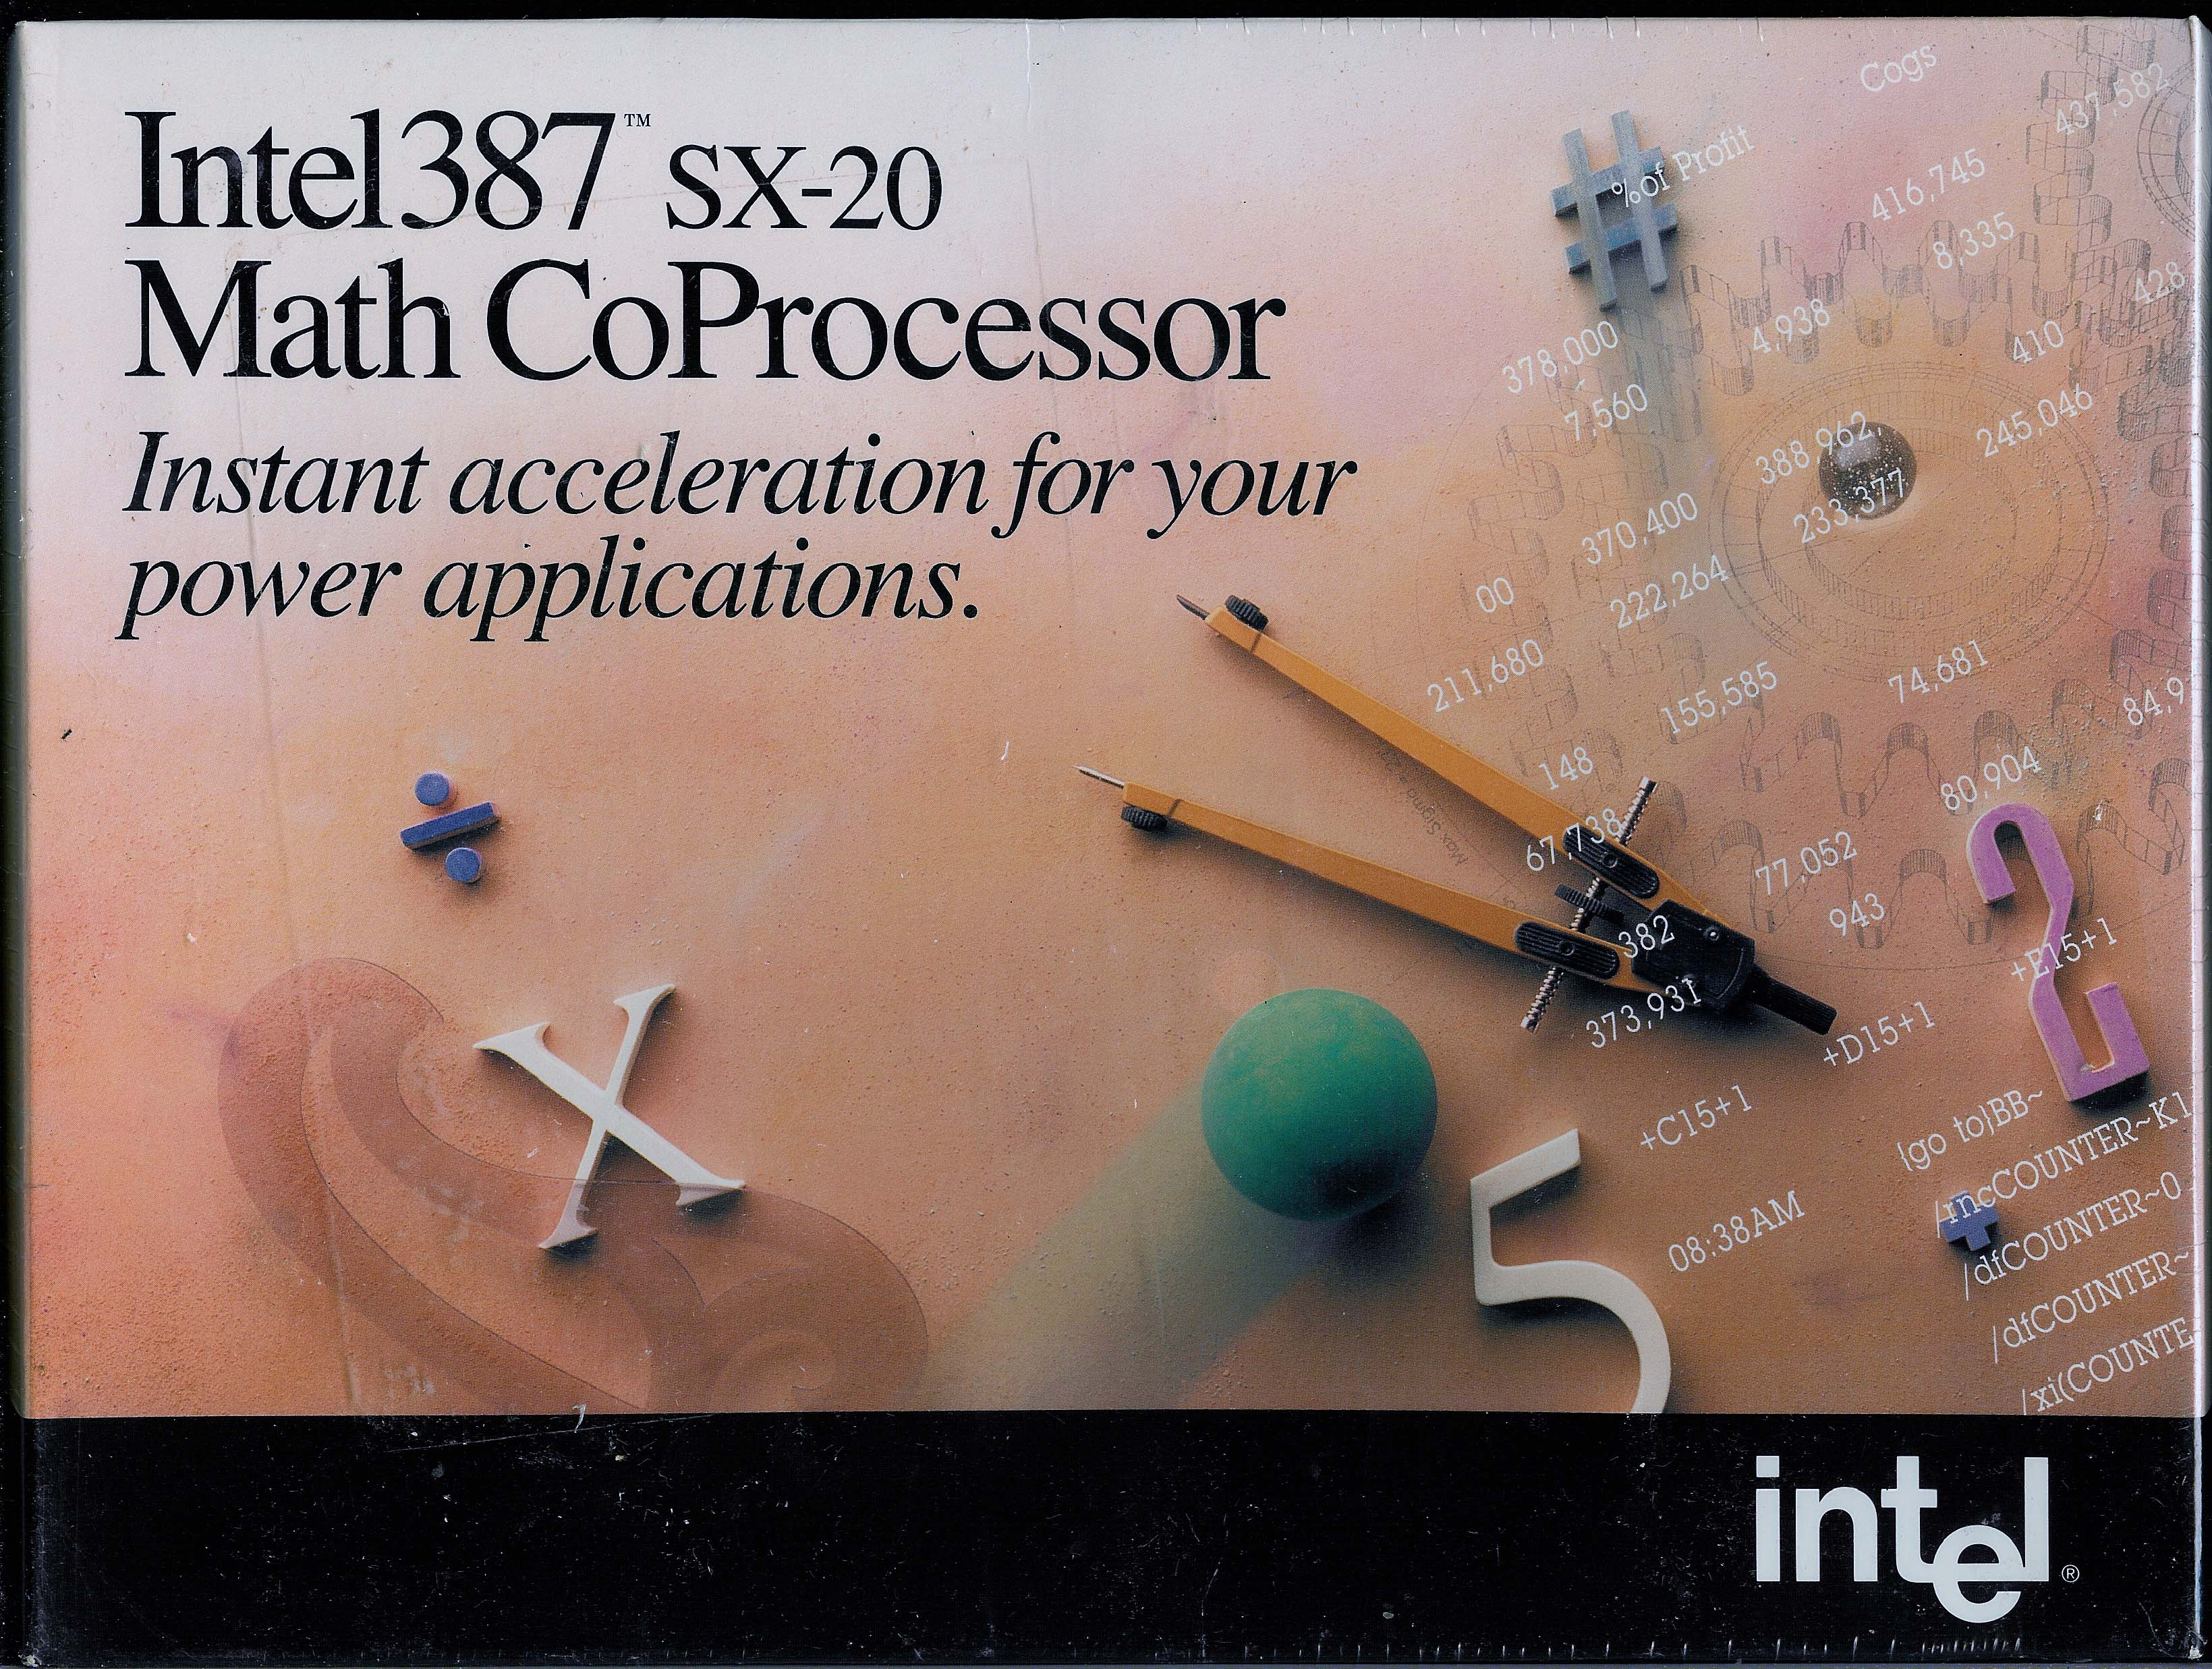
\includegraphics[scale=0.5]{imgs/BOX_IntelBOX387SX20.jpg}
  }
\caption{Intel 1991 ad for "Math CoProcessor".}
\label{fig:fp_internals}
\end{figure}



\bigskip
This concludes the CPU stage of the pipeline, in a rather pessimist way: At first sight, 286 and 386 \emph{int} operations were fast but not accurate enough and \emph{float} operations were accurate but not fast enough. It looked like there was not way to do real-time trigonometry.

   















\section{RAM}
The target machines could have their CPU set in two modes:
\begin{itemize}
  \item The new Protected Mode was the last addition of Intel with an address bus 32 bits wide and a MMU\footnote{Memory management Unit} offering up to 4 GB of memory protected linear RAM.
  \item The Real Mode was \emph{just} a backward compatibility mode so old software written for 8086 from the 70s could still run. 
\end{itemize}
  You may assume that programers of the 90s switched the CPU in Protected Mode to unleash the full potential of the machines. Unfortunately, there was a major obstacle between this nice feature and the programmer. The infamous operating system, MS-DOS 5.0 by Microsoft Corporation.
  






  \subsection{DOS limitations}
  Microsoft Corporation highly valued the applications running on their operating systems. They were adamant to never ever break anything with a new system.  Since many applications were written during the 80s on machine having only Real-Mode, DOS 5.0 kept running that way and as a result its routines were incompatible with Protected Mode. This created an awkward situation where the \emph{de-facto} operating system that came with every machine sold prevented programmers from using Protected Mode. They were forced to ignore all the neat features of their 1992 PC and use the machine like it was a very fast Intel 8086 CPU from 1976.

\bigskip

 \textbf{\underline{Trivia :}} One year earlier, in 1991, a student from the University of Helsinki started working on a "hobby" of his: An operating system able to use the CPU in Protected Mode taking advantage of the MMU and the 32 bits registers. It would become Microsoft worse nightmare. Linus Torvalds had just started what would become Linux.



  \subsection{The infamous Real Mode: 1MB RAM max}
  Protected mode was unavailable. What had the Real-Mode to offer ? Essentially a trip back in time to 1976: A 20 bits wide address bus offering only 1MB of addressable RAM. No matter how much memory was installed on the machine in 1992, only 1MB could be addressed. And to top it all, addressing had to be done not with the 32 bits registers available but by combining two 16 bits register together: One was the segment, the other an offset within that segment. Hence the name: '16 bits programming'.

  \bigskip
Here is a brief description of the memory layout: \\
\begin{itemize}
\item From 00000h to 003FFh : the Interrupt Vector Table.
\item From 00400h to 004FFh : BIOS data.
\item From 00500h to 005FFh : command.com+io.sys.
\item From 00600h to 9FFFFh : Usable by a program (around 620KB). 
\item From A0000h to FFFFFh : UMA (Upper Memory Area): Reserved to bios ROM, video card and sound card mapped I/O.
\end{itemize}

\begin{figure}[H]
\centering
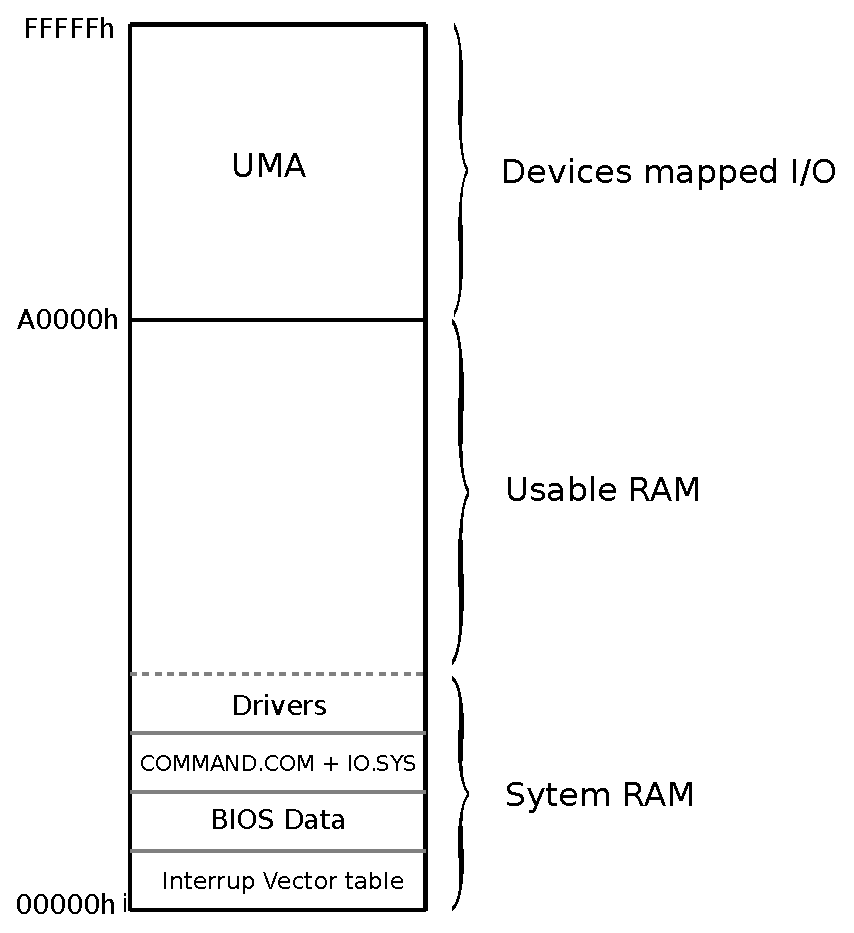
\includegraphics[scale=1]{imgs/real_mode}

\caption{3.14 window and offset.}
\label{fig:fp_internals}
\end{figure}


As a result, out of the original 1024KB, only 640KB (called Conventional Memory) were usable. 384KB were reserved for the UMA\footnote{Upper Memory Area} and every single driver installed (\codeword{.SYS} and \codeword{.COM})  took away from the remaining 640KB.

\bigskip

\textbf{\underline{Trivia :}}  In France people had to load KEYBFR.SYS driver so their AZERTY keyboard keys woud be properly mapped. The driver consumed a whopping 5KB of Conventional Memory.\\
\\

\subsection{The infamous Real Mode: 16 bits Segmented addressing}
Real Mode could not use 32 bits registers for addressing. Everything had to be done by combining two 16 bits registers as seen in Figure \ref{fig:register_comb_to_20_bits}. There were two kinds of RAM pointers: near and far. In the case of a far pointer, a 16 bits segment register would be shifted left 4 bits and combined with an other 16 bits offset register\\
\begin{figure}[H]
\centering
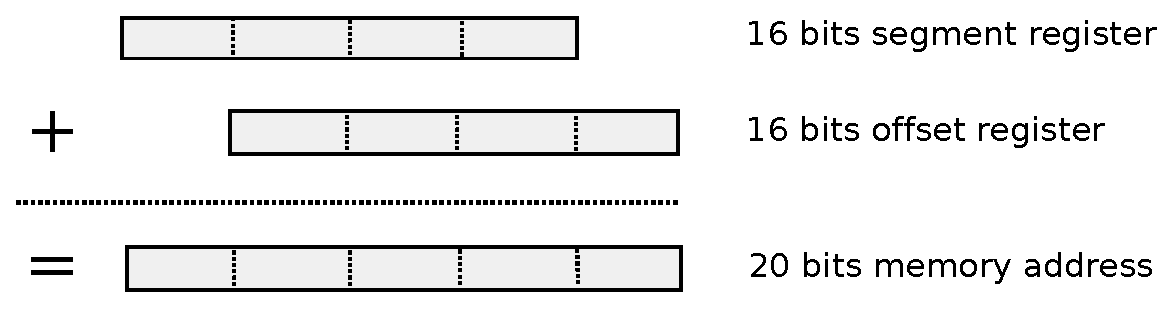
\includegraphics[scale=0.8]{imgs/register_combination_20_bits_address.eps}
\caption{How registers were combined to address memory.}
\label{fig:register_comb_to_20_bits}
\end{figure}
A near pointer was just a 16 bits offset that would point in the same segment.\\  
\bigskip
That may not sound too bad but in practice this segmented addressing led to many issues:
\bigskip
The least probemetatic was about the langauge: Since the C language was invented on 32 bits machine, the language had to be augmented by compiler manufacturers. That is how the \codeword{near} and \codeword{far} keywords came to existence. To build pointers, a set of macro would be provided, respectively \codeword{FP\_SEG} and \codeword{FP\_OFF}.\\
\\
But the really big issue was how two pointers, refering to the same address could fail an equality test: In this model, the 1MB of RAM is divided in 65536 paragraphs by the segment pointer. So a paragraph is 16 bytes but an offset can be up to 65536 !!! See the following example:\\
\bigskip
\\Pointer A defined as:
\begin{Verbatim}[fontsize=\relsize{-1}]
    0000 0000 0000 0000 0000  Segment, 16 bits shifted 4 bits left  
  +      0000 0001 0010 0000  Offet,   16 bits
============================
    0000 0000 0001 0010 0000  Address, 20 bits
\end{Verbatim}

\bigskip

Pointer B defined as:
\begin{Verbatim}[fontsize=\relsize{-1}]
    0000 0000 0001 0000 0000  Segment, 16 bits shifted 4 bits left  
  +      0000 0000 0010 0000  Offet,   16 bits
============================
    0000 0000 0001 0010 0000  Address, 20 bits
\end{Verbatim}

\bigskip

Pointer C defined as:
\begin{Verbatim}[fontsize=\relsize{-1}]
    0000 0000 0001 0010 0000  Segment, 16 bits shifted 4 bits left  
  +      0000 0000 0000 0000  Offet,   16 bits
============================
    0000 0000 0001 0010 0000  Address, 20 bits
\end{Verbatim}

As defined A, B and C all points to the same memory location however they would fail a comparison test in the following code.\\

\lstinputlisting[language=C]{code/pointer_madness.c}

Woud ouput:


\lstinputlisting{code/pointer_madness_output.txt}

\bigskip





  \subsection{Extended Memory}

The 20 bits address but of Real Mode limited the addressable RAM to 1MB. But machines of 1992 came equipped with more, typically 2MB and even sometimes 4MB. The workaround at the time was to install special drivers that would open a window beyond the addressable RAM as shown in Figure \ref{fig:ems_xms_layout}.

\begin{figure}[H]
\centering
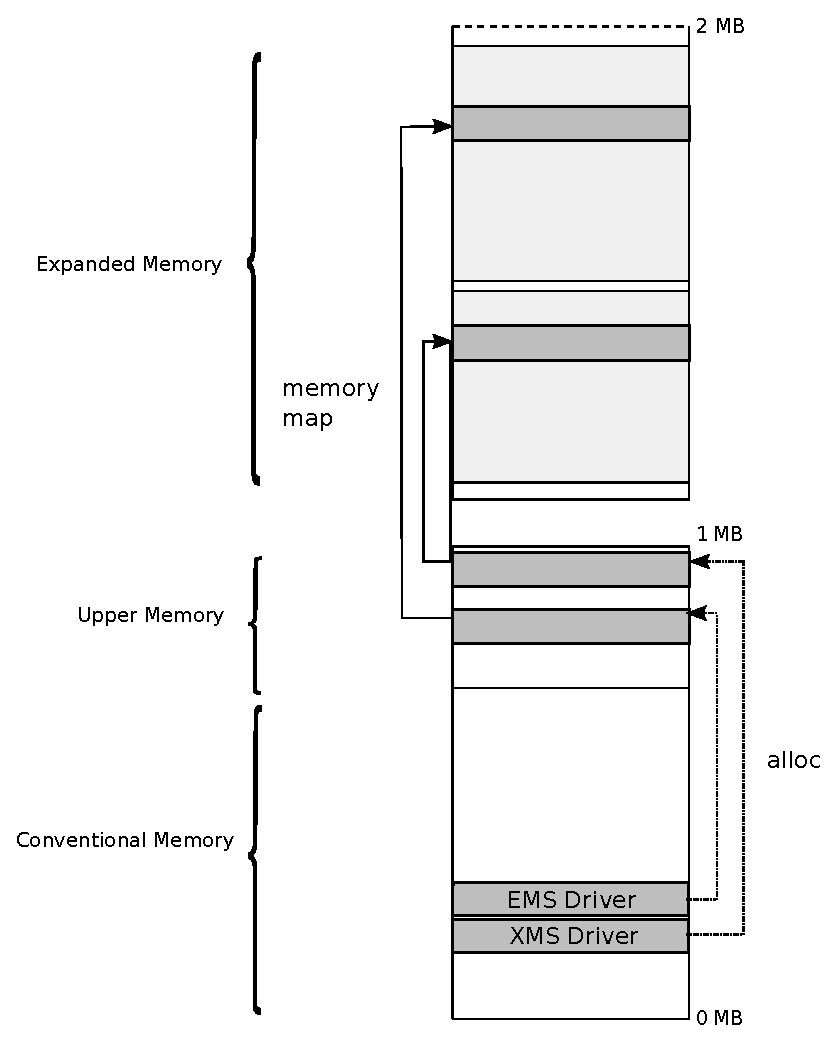
\includegraphics[scale=1]{imgs/expanded_ram.eps}
\caption{Expanded memory layout}
\label{fig:ems_xms_layout}
\end{figure}

Unfortunately once again, nothing was standardized. Users could load different drivers:
\begin{itemize}
\item Expanded Memory Specification (EMS) drivers: EMM368.SYS.
\item eXtended Memory Specification (XMS) drivers: HIMEM.SYS .
\end{itemize}

Or they could decide to load no drivers at all at startup and not use any of the RAM beyond 1MB.\\
\textbf{\underline{Trivia :}}  This 640KB barrier was a big issue. Many customer could not understand why even though they had many MB installed on their machine, some game would refuse to start up claiming "Not enough memory". id Software had to publish an explanation (Appendice "\nameref{chap:barrier640}") along with the game to make it clear that it was not their fault.

{\underline{Trivia :}}  As of 2014, thirty five years after the introduction of the 8086, most PC in the world start in  real mode. Then a bootloader switch them to protected mode, load the kernel and then real startup can begin. Mac computers don't have this problem.

\bigskip

{\underline{Trivia :}}  As of 2014, thirty five years after the introduction of the 8086, most PC in the world still use segmented addressing.\\

Include reference to XMS and EMS programming reference. \footnote{eXtended Memory Specification (XMS) July 19, 1988.}


\section{Video}

PC were connected to a CRT monitor: Huge, cathodic ray based, small screen, curved surface, deep and incredibly heavy devices. Most monitor had a tiny 13" diagonal with a 4:3 aspect ratio. Figure \ref{fig:int_layout} shows a comparison between a monitor of 1992 and a 28" LCD display from 2014.\\

\begin{figure}[H]
\centering
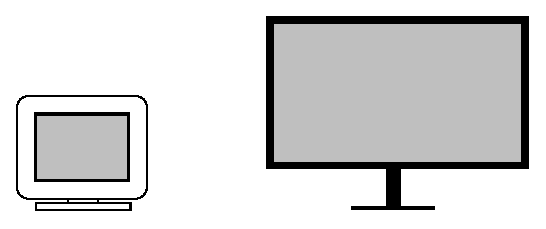
\includegraphics[scale=1.2]{imgs/crt_lcd.eps}
\caption{CRT vs LCD screen surfaces.}
\label{fig:lcd_vs_crt}
\end{figure}

{\underline{Trivia :}} How big and heavy could a CRT be ? The InterView 28hd96 by Integraph weighted 45kg (99.5lb). For comparison, a modern DELL LCD 27" weights 7.8kg (17lb).
\bigskip
Since the monitor were analogic and the PC were digital, there had to be an interface between the two. They were called Adapters.

  \subsection{History}

From 1981onward, many systems were released:
\bigskip
  
 \begin{figure}[H]
\centering  
\begin{tabularx}{0.9\textwidth}{ X  Y }
  \toprule
  \textbf{Name} &  \textbf{Year Released} \\
  \toprule \codeword{MDA}
   (\textbf{M}onochrome
   \textbf{D}isplay
   \textbf{A}dapater) & 1981 
   \\ \codeword{CGA}
   (\textbf{C}olor
   \textbf{G}raphics
   \textbf{A}dapter) & 1981 
    \\ \codeword{EGA}
   (\textbf{E}nhanced
   \textbf{G}raphics
   \textbf{A}dapter) & 1985
   \\ \codeword{VGA}
   (\textbf{V}ideo
   \textbf{G}raphics
   \textbf{A}rray)  & 1987
    \\
  \toprule
\end{tabularx}
\caption{Video interface history.}\label{fig:vga_history}
\end{figure}

Each added new feature to the previous iteration. In 1993 the ubiquitous graphic system was the VGA\footnote{Video Graphic Adapter}. The universality of that system was a two edged sword: One one side developers did not have to deal with hereogeneity. But on the other side, the shortcoming of the Adapater were the same for everybody.\\

In 1993, the VGA (Video Graphic Array) was the chipset in charge of interfacing the CPU and the CRT.


\subsection{VGA Architecture}

That chip was a blessing and a curse: It was universally deployed on every single IBM PC on the market but it was also poorly documented and complicated to program with more than 300 internal registers.\\
\bigskip
  Three parts were interacting around 256Kb of RAM:

\begin{itemize}
\item The Graphic Controller and Sequence Controller controlled how the RAM was populated.
\item The RAM stored the framebuffer.
\item The CRTC Controller and the DAC (Digital To Analog Converter) took care of converting the framebuffer to analogic signal.
\end{itemize}



\begin{figure}[H]
\centering
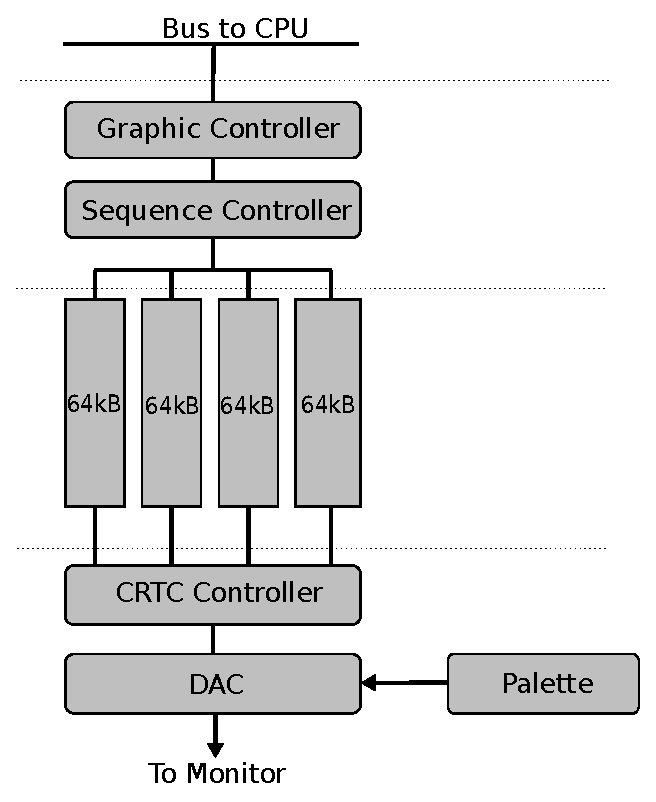
\includegraphics[scale=1.2]{imgs/vga.eps}
\caption{Video Graphic Array Architecture.}
\label{fig:vga_arch}
\end{figure}



The most surprising part of the architecture is the framebuffer (the RAM that contain the image before it is sent to the screen) which is not one big linear array but four parallel memory banks (called planes). The design raison d'etre was twofold :



\begin{itemize}



\item Backward compatibility: EGA (the precursor of VGA) had only 64kB of RAM. It was easy to emulate EGA by using only one bank.
\item Hardware limitations: A CRT running at 60Hz and displaying 640x480 needed a pixel every 1/(640*480*60)th of second . That mean one pixel each 54ns. The problem was the RAM access time was 200ns so that was not possible. But if latency could not be reduced, the throughput could be improved by fetching 1 pixel + 3 others in advance. Therefore the memory banks were read in parallel: 4 bytes at a time and the CRTC had an amortized latency of 200/4 = 50ns/pixel which was fast enough.
\end{itemize}


\subsection{VGA Planar madness}

This bandwidth limitation led to bizarre things. The main one is that data could not be stored linearly and sent to the screen. Because memory was read 4 bytes at a time but from four planes, the layout looked like this:\\

\begin{figure}[H]
\centering
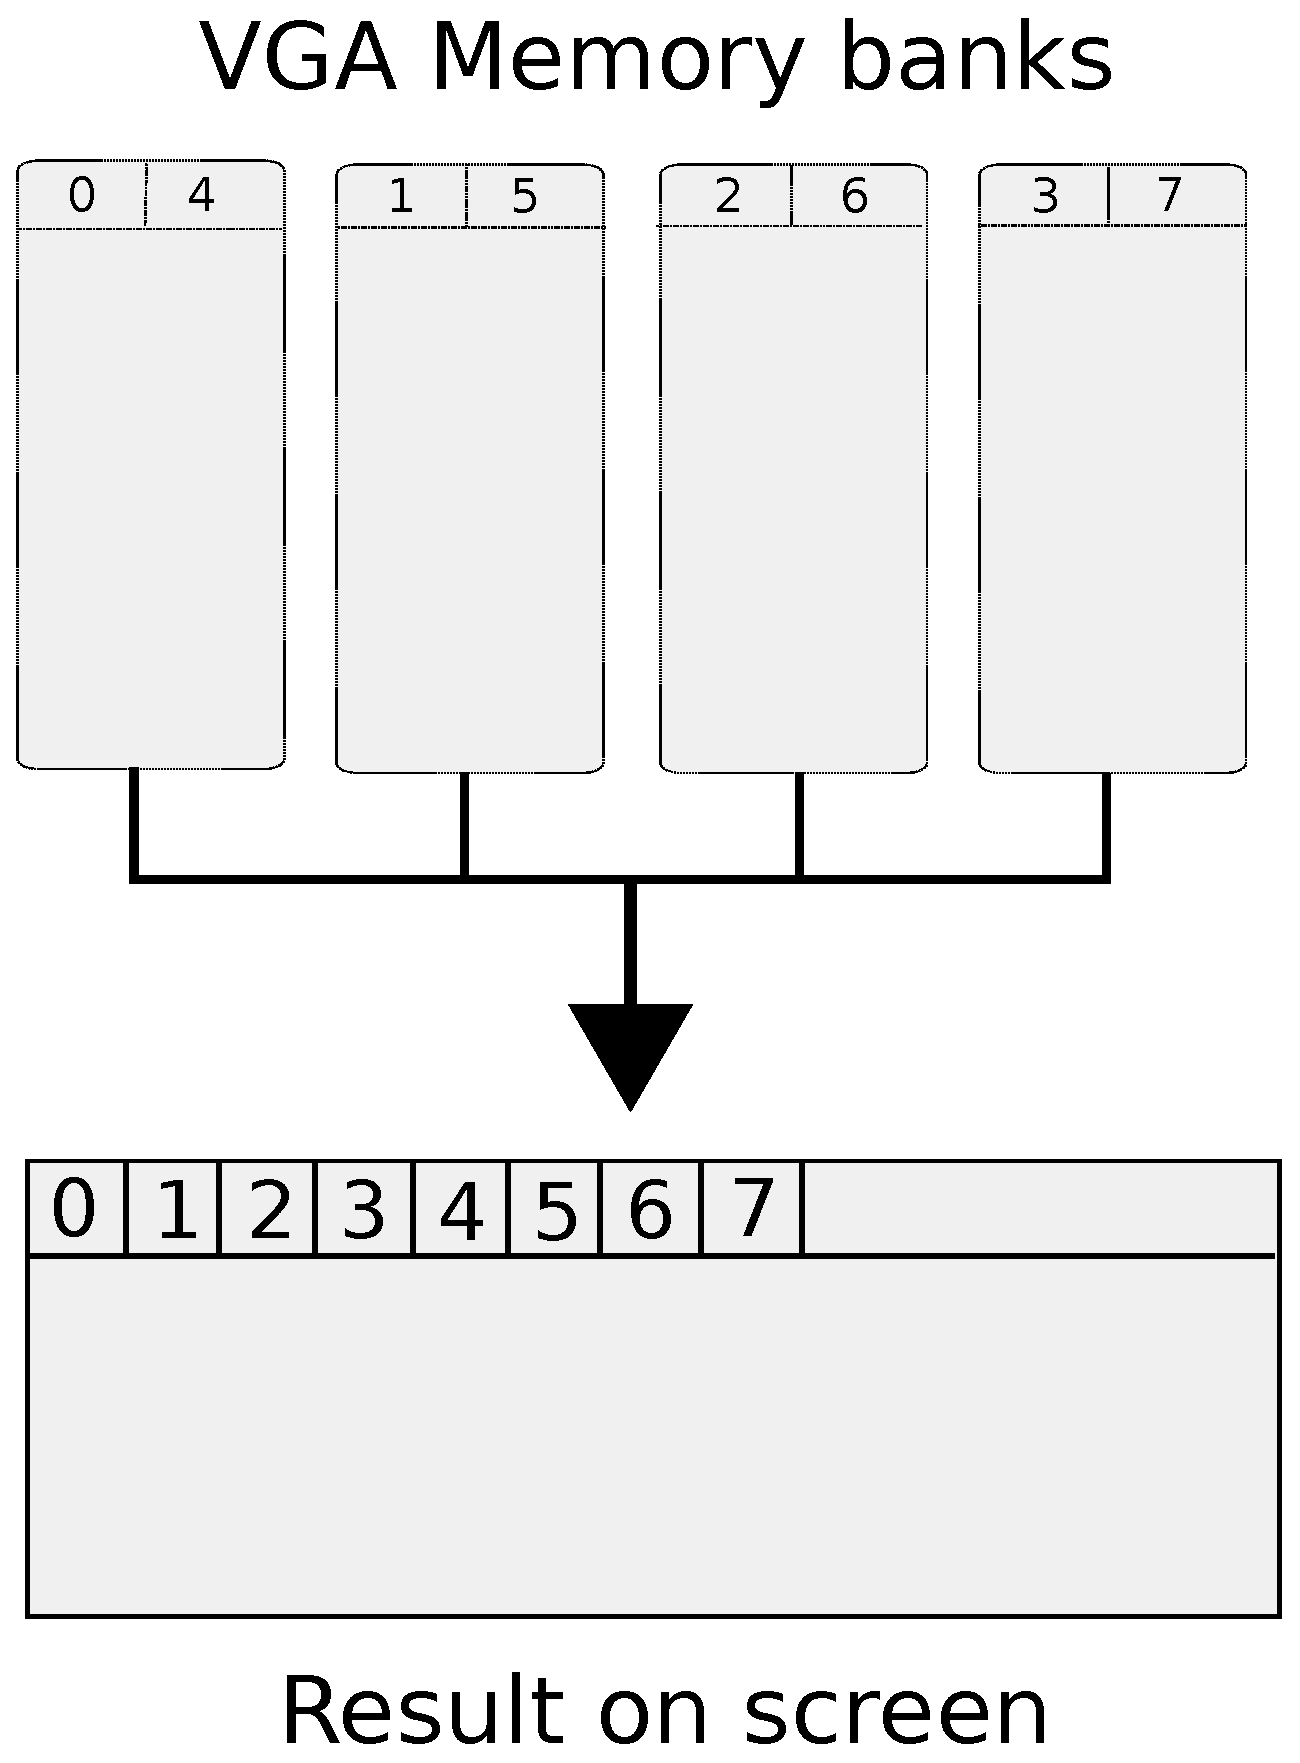
\includegraphics[scale=0.5]{imgs/vga_ram_screen_layout.eps}
\caption{Video Graphic Array Architecture.}
\label{fig:vga_arch}
\end{figure}

 {\underline{Note :}} The clean pipeline architecture in Figure \ref{fig:vga_arch} is an oversimplication. In reality each Controller interacted with the rest of the system. The actual drawing, staight from IBM VGA Reference looks like this:\\
 
 
 \begin{figure}[H]
\centering
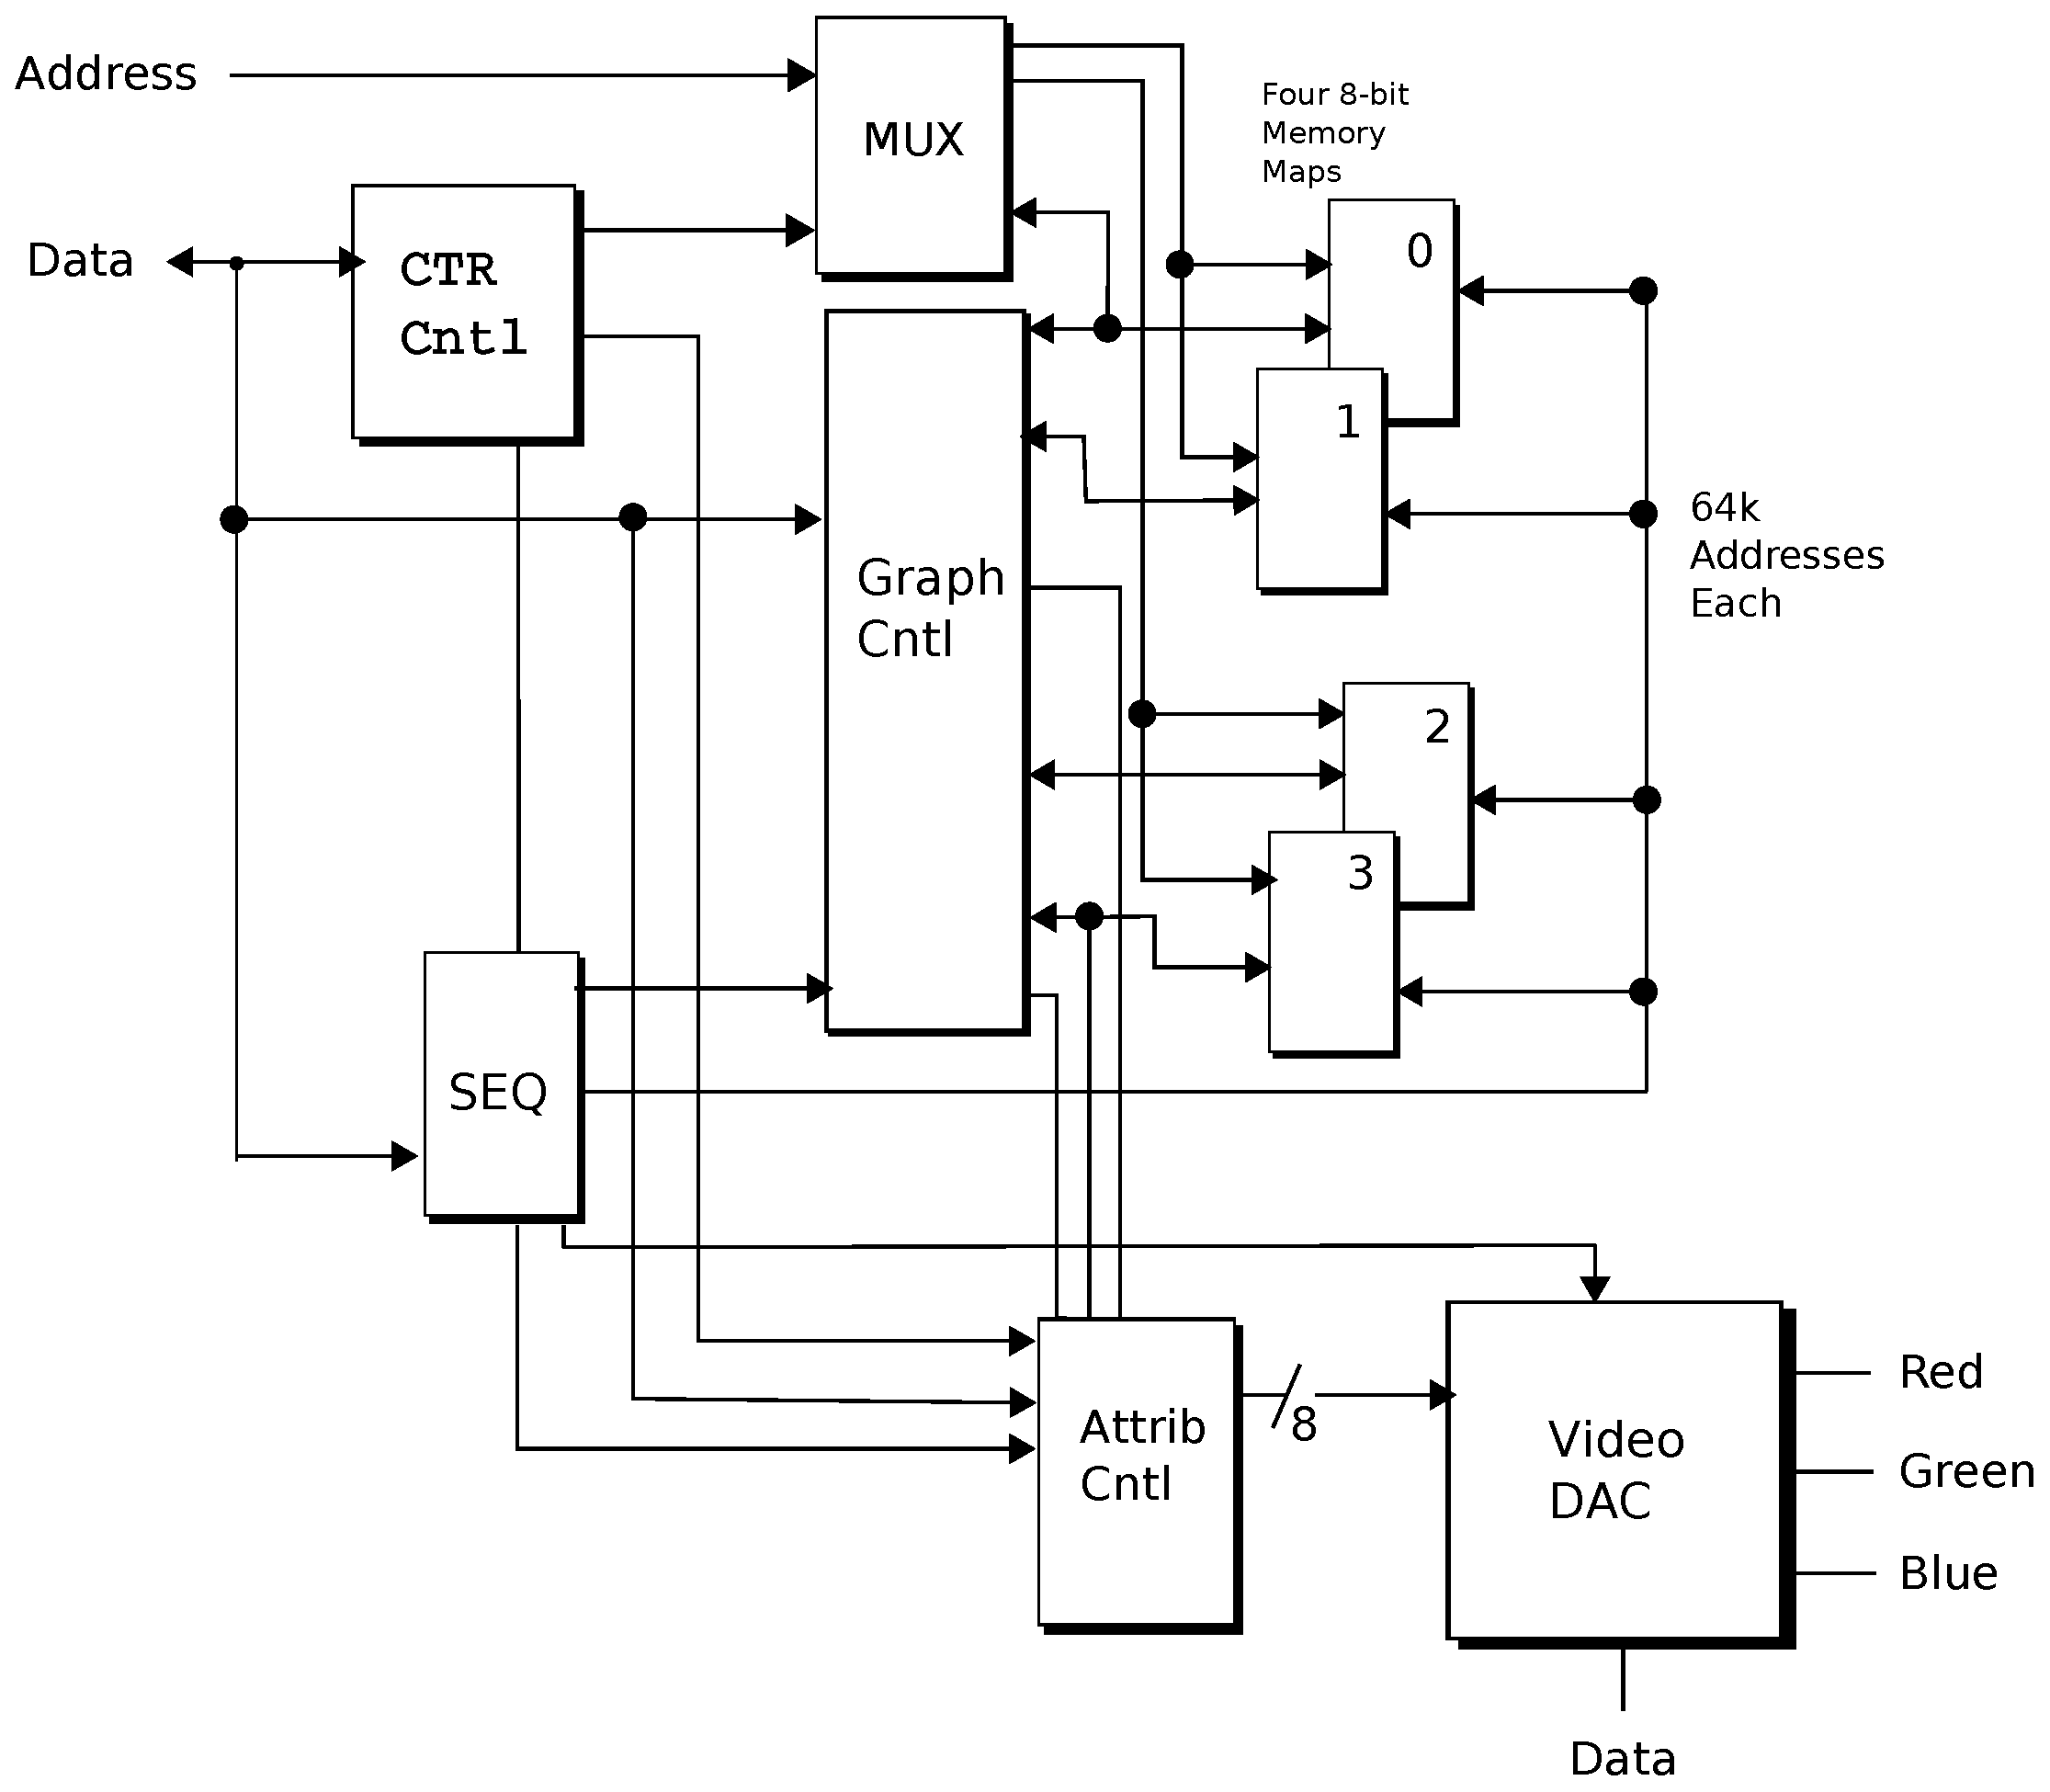
\includegraphics[scale=0.38]{imgs/ibm_vga.eps}
%\def\svgscale{1.5}
%\input{imgs/fun_pipeline.pdf_tex}
\caption{IBM's VGA Documentation}
\label{fig:ibm_vga}
\end{figure}

\bigskip
To configure this mess of planes, registers and controllers meant setting up more than 300 registers to interact together. Needless to say few programmers got to dive in the internal of this thing. Luckily IBM BIOS had a few preset configutation (called "mode") with an associated resolution and color numbers.

\subsection{VGA Modes}

The BIOS could be called to have the VGA configured with preset registers.

\begin{figure}[H]
\centering
\begin{table}[H]
\begin{tabular}[c]{llllr}
\hline
\textbf{Mode} & \textbf{Type} & \textbf{Format} & \textbf{Colors}          & \multicolumn{1}{l}{\textbf{Segment}} \\ \hline
0             & text          & 40x25           & 16 gradient (monochrome) & b800h                                \\ \hline
1             & text          & 40x25           & 16                       & b800h                                \\ \hline
2             & text          & 80x25           & 16 gradient (monochrome) & b800h                                \\ \hline
3             & text          & 80x25           & 16                       & b800h                                \\ \hline
4             & CGA Graphics  & 320x200         & 4                        & b800h                                \\ \hline
5             & CGA Graphics  & 320x200         & 4 gradient (monochrome)  & b800h                                \\ \hline
6             & CGA Graphics  & 640x200         & 2                        & b800h                                \\ \hline
7             & MDA text      & 9x14            & 3 gradient (monochrome   & b000h                                \\ \hline
0Dh           & EGA graphic   & 320x200         & 16                       & A000h                                \\ \hline
0Eh           & EGA graphic   & 640x200         & 16                       & A000h                                \\ \hline
0Fh           & EGA graphic   & 640x350         & 3                        & A000h                                \\ \hline
10h           & EGA graphic   & 640x350         & 16                       & A000h                                \\ \hline
11h           & VGA graphic   & 640x480         & 2                        & A000h                                \\ \hline
12h           & VGA graphic   & 640x480         & 16                       & A000h                                \\ \hline
13h           & VGA graphic   & 320x200         & 256                      & A000h                                \\ \hline
\end{tabular}
\end{table}
\caption{VGA Modes available from BIOS.}\label{fig:vga_modes}
 \end{figure}
 
The best was of course....13h and 12h

 \begin{fancyquotes}
   Right off the bat, I'd like to make one thing perfectly clear: The VGA is hard-sometimes very hard-to program for good performance.
 \bigskip \\
\textbf{Michael Abrash - Zen VGA guru}
 \end{fancyquotes}
 
 



 
 
  \subsection{VGA Programming}
  Using the VGA as per the manual is easy. A few instructions are enough to call the BIOS and setup the environment. The most appealing mode for game is of course 320x200 256 palettes based color: Mode 13h.\\
  \lstinputlisting[ language={[x86masm]Assembler}]{code/vga_mode13.asm}
  The \codeword{int 10} instruction is an interrupt calling BIOS routine. It looks up the \codeword{ax} register to load the requested mode.\\
  
  After setting up the VGA, the programmer has access to a linear framebuffer of 64KB mapped at \codeword{A0000h}.\\
  
  DRAWING
  
  To clear the screen to black for example, the following code was enough:\\
  
  \lstinputlisting[language=C]{code/clear_vga.c}
  
  
  The mode 13h may look good but it is in fact terrible for game and animation. The intend was clearly to display static images:
  \begin{itemize}
\item All the RAM is used and there is no way to have a double buffer.
\item Since the resolution is 320x200, the aspect ration does not feet the monitor. As a result the image is streched when transfered from the 
framebuffer to the CRT.

 \begin{figure}[H]
\centering
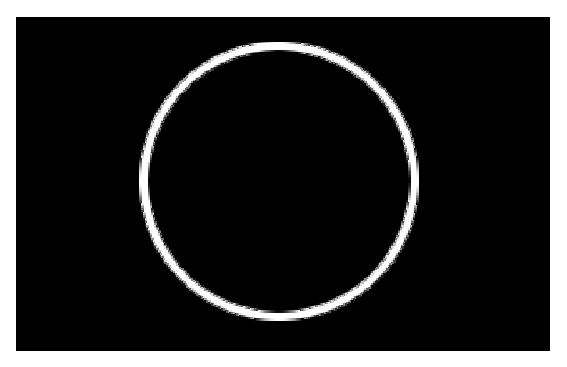
\includegraphics[scale=1.0]{imgs/circleframebuffer.eps}
%\def\svgscale{1.5}
%\input{imgs/fun_pipeline.pdf_tex}
\caption{Parallele Port}
\label{fig:parallelPort}
\end{figure}

 \begin{figure}[H]
\centering
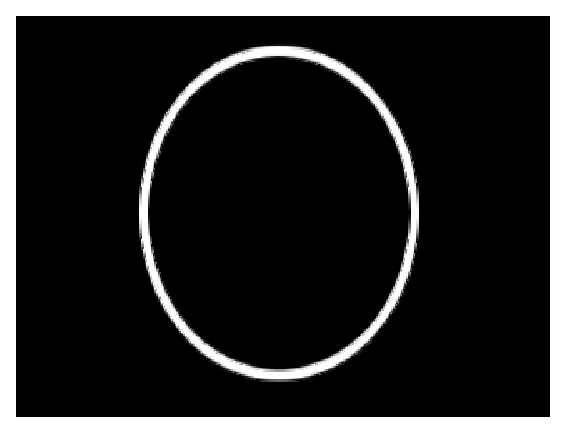
\includegraphics[scale=1.0]{imgs/circlescreen.eps}
%\def\svgscale{1.5}
%\input{imgs/fun_pipeline.pdf_tex}
\caption{Parallele Port}
\label{fig:parallelPort}
\end{figure}

\item VGA MAPPING I/O WASTED SPACE.

\end{itemize}





  

\section{Audio}
Off all the parts in a PC, the audio system was the best. The card manufacturer had started to see a market and player actually had the opportunity to buy decent stuff.
  \subsection{Speaker}
  PC came out of the box with a binary beeper. I was able to produce two frequency.
  \subsection{Ad Lib}
  Canadian manufacturer of sound cards
  Music (midi)
  Not about canada: adlib, watcom and matrox millenium
  \subsection{Sound Blaster}
  The Sound Blaster 1.0 (code named "Killer Kard"),[1] CT1320A, was released in 1989
  Music (midi+digitized sound)]  But it also added two key features absent from the Adlib: a PCM audio channel, and a game port.
  \subsection{Sound Blaster Pro}
  Model CT1330, announced in May 1991, was the first significant redesign of the card's core features, and complied with the Microsoft MPC standard.[6]. The Sound Blaster Pro supported faster digital sampling rates (up to 22.05 kHz stereo or 44.1 kHz mono), added a "mixer" to provide a crude master volume control (independent of the volume of sound sources feeding the mixer), and a crude high pass or low pass filter. The Sound Blaster Pro used a pair of YM3812 chips to provide stereo music-synthesis (one for each channel).
\section{Inputs}
Inputs were a mess. This was time before USB. Each peripheric was using a differnt port.

The parallel port was usually used for printers.
 \begin{figure}[H]
\centering
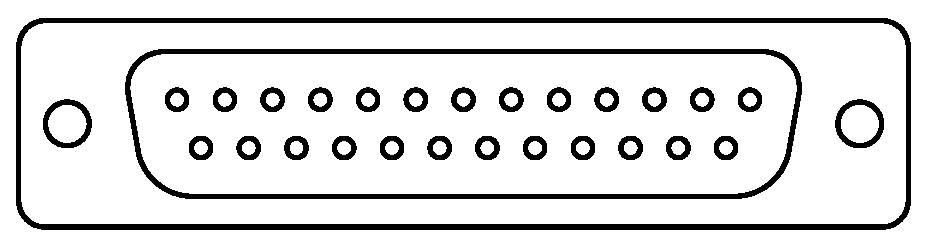
\includegraphics[scale=0.7]{imgs/ports/DB-25_parallel_port.eps}
%\def\svgscale{1.5}
%\input{imgs/fun_pipeline.pdf_tex}
\caption{Parallele Port}
\label{fig:parallelPort}
\end{figure}


The serial port was used to connect the mouse.
 \begin{figure}[H]
\centering
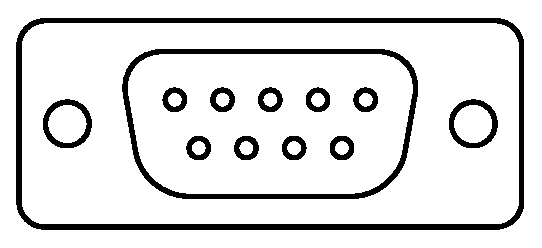
\includegraphics[scale=0.7]{imgs/ports/DE9_serial_port.eps}
%\def\svgscale{1.5}
%\input{imgs/fun_pipeline.pdf_tex}
\caption{Serial Port}
\label{fig:serialPort}
\end{figure}

The keyboard was using something different: a PS/2 port.
 \begin{figure}[H]
\centering
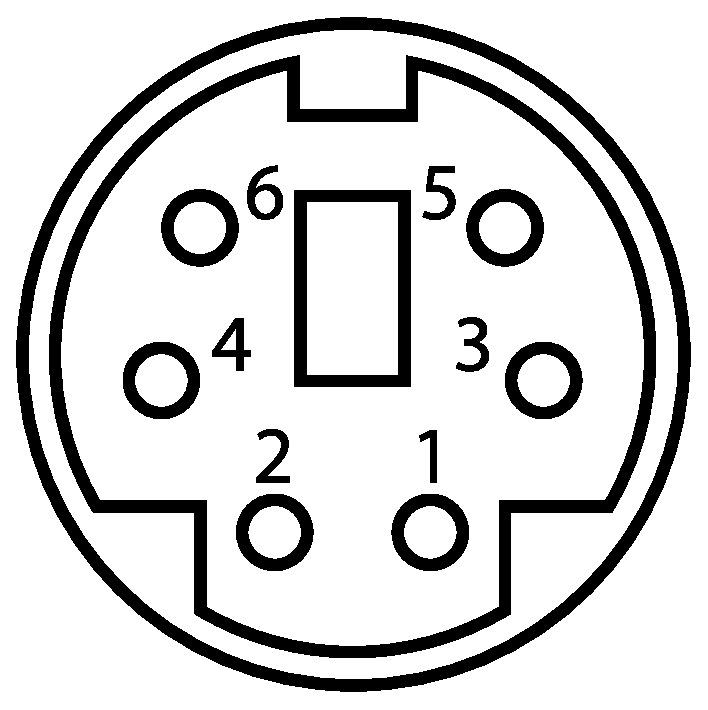
\includegraphics[scale=0.2]{imgs/ports/MiniDIN-6_PS2.eps}
%\def\svgscale{1.5}
%\input{imgs/fun_pipeline.pdf_tex}
\caption{PS/2 Port}
\label{fig:ps2Port}
\end{figure}


Finally, sound card connected via the ISA bus provided a Game Port allowing to connect a joystick.
 \begin{figure}[H]
\centering
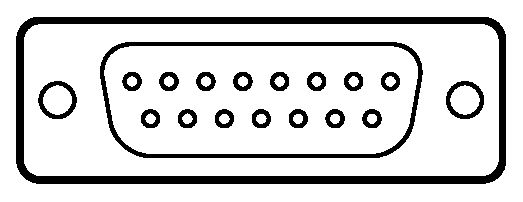
\includegraphics[scale=0.9]{imgs/ports/DA-15_GamePort.eps}
%\def\svgscale{1.5}
%\input{imgs/fun_pipeline.pdf_tex}
\caption{Game Port}
\label{fig:gamePort}
\end{figure}

Note that without a sound card you were unable to connect a joystick !



\section{Summary}
I hope this summarize well that the hardware sucked for what id Software intended to do. 

\end{document}




